\documentclass[12pt]{article}

\usepackage[utf8]{inputenc}
\usepackage{float}
\usepackage[colorlinks,citecolor=blue,urlcolor=blue]{hyperref}
\usepackage[pdftex]{graphicx}
\usepackage{parskip}
\usepackage{subfig}
% \usepackage{fullpage}
\usepackage{amsmath}
\usepackage{amssymb}
\usepackage{color}
\usepackage{todonotes}
\usepackage{listings}
\usepackage{common}
\usepackage{bm}
\usepackage{enumitem}
\usepackage{tikz}
\usepackage{soul}
\usepackage{framed}
\usepackage{pythonhighlight}
\usepackage{common}
\usepackage{booktabs}

\title{Supervised Machine Learning for Biomolecular Condensate Quantification and Measurement}
\author{AM91r: Supervised Reading and Research
\\ Rodney Lafuente Mercado 
\\ lafuentemercado@college.harvard.edu}
\date{May 4, 2022}


\begin{document}


\maketitle{}

\begin{abstract}
\noindent This report covers an application of supervised machine
learning for to the identification of biomolecular condensates in SARS-CoV-2 nucleocaspids. The
report covers feature and model selection as well as masking and segmentation for differentiation
of condensates respective to the cells in which they are located, their intensities, and their areas.

\end{abstract}

\section{Background}

The motivation behind this project is to quantify the effect of different compounds on condensate
formation in SARS-CoV-2 nucleocaspids. Alternatives to machine learning for blob detection consist
of filtering and thresholding techniques that alter cell images depending on desirable properties.
The method outlined in this paper is inspired by Ilastik$^1$, a pixel classification tool using that
uses ensemble methods and differing image filters. Images analyzed in this project were of cells in
different stained environments. The data set analyzed in this project contained three different
wavelengths for each image, each corresponding to a different goal. These are visualized in
Figure~\ref{fig:wavelengths} for an example well site.

\begin{figure}[H]
    \centering
    {
        \subfloat[Hoechst stain]{
            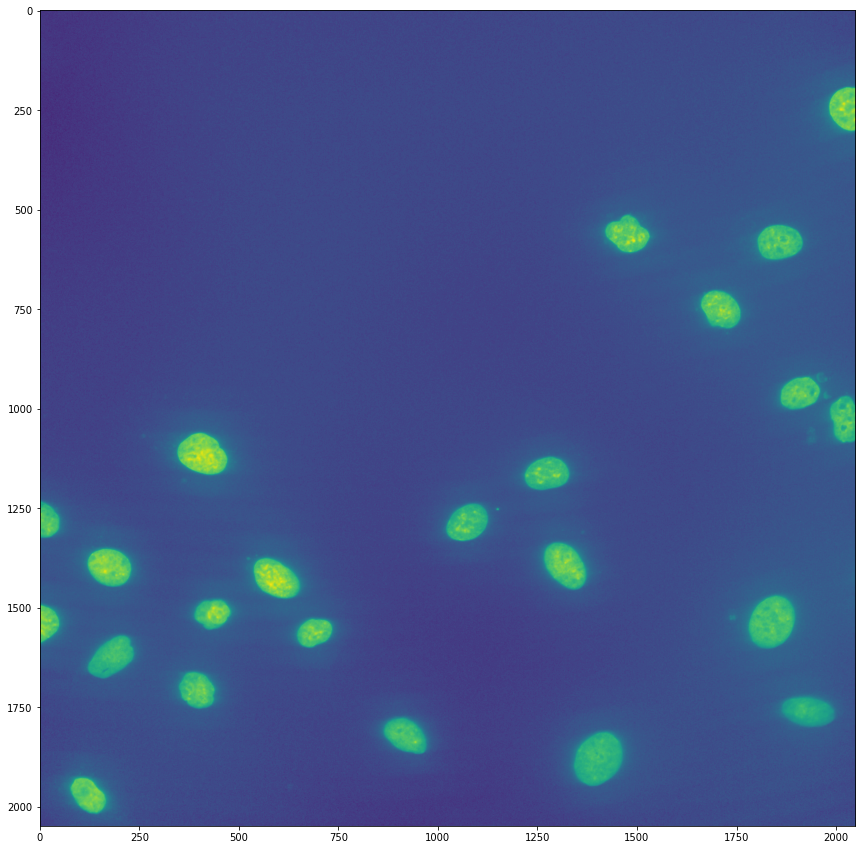
\includegraphics[width=0.3\textwidth]{wavelength_1.png}
        }
        \subfloat[GFP]{
            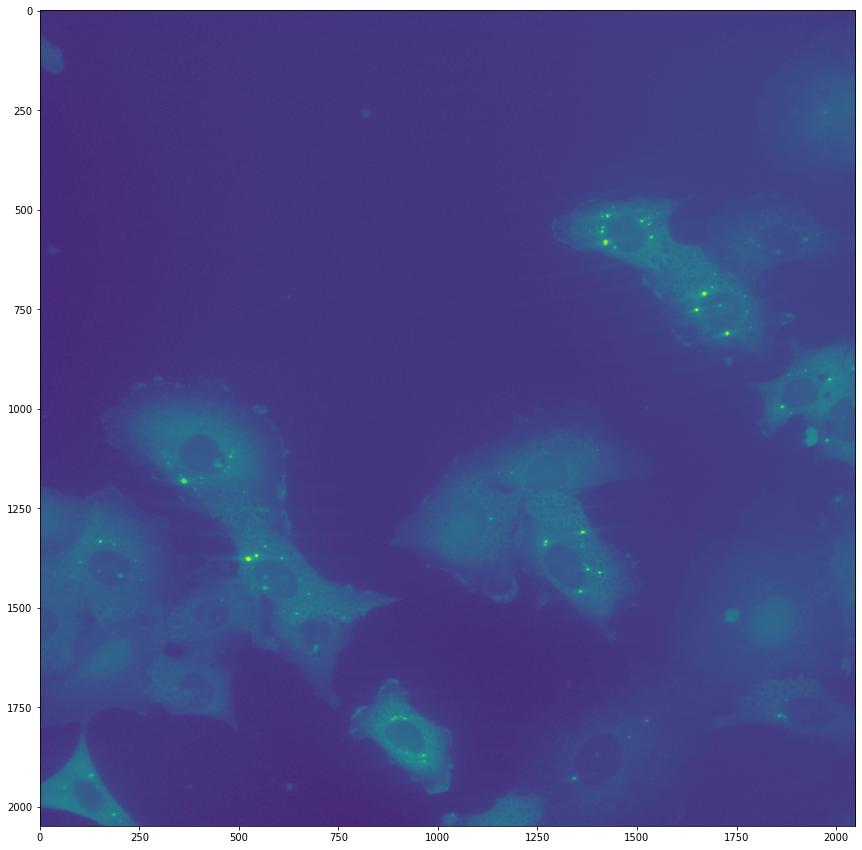
\includegraphics[width=0.3\textwidth]{wavelength_2.png}
        }
        \subfloat[CellMask]{
            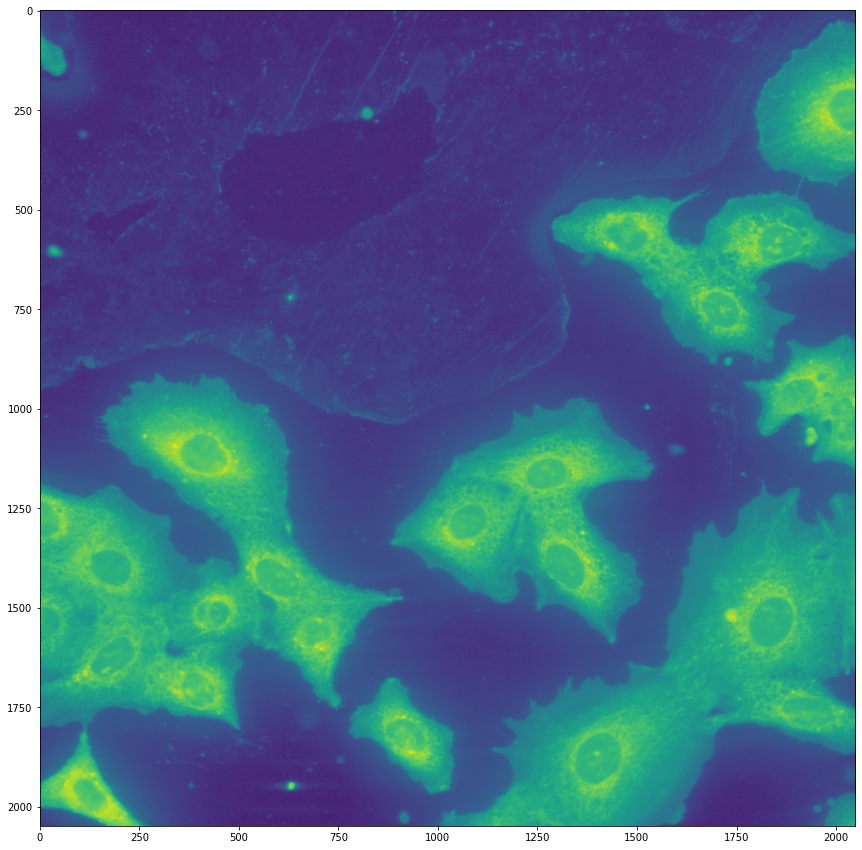
\includegraphics[width=0.3\textwidth]{wavelength_3.png}
        }
    }\caption{Example of Well Site Wavelengths}
    \label{fig:wavelengths}
\end{figure}

Each of these wavelengths is used for a different goal, with the GFP wavelength being the most 
important for the purposes of pixel classification, as it contains information on condensates
as visibly brighter, circular blobs. The other two wavelengths are used in segmenting the cells
and removing anomalies in the images posterior to pixel classification.

\section{Cell Segmentation}

Cell segmentation in this project was required in order to determine what blobs belonged to which cells. 
A mask is required to accomplish this, which is an array of the same size of the images (2048 by
2048) with zeroes representing background areas (e.g., pixels not part of any cells) and integers
for each different cell. After pixel classification is performed on the wavelength containing
information on condensates (GFP), the condensates are filtered and counted using this mask. 

Figure~\ref{fig:masking_process} demonstrates the masking process, which consists of finding nuclei,
findingn cytoplasm, and combining these two images to segment the cells using a watershed algorithm.
The watershed algorithm takes as input binary images that it treats as topological maps such that
they are flooded in order to find the proper separation between regions. This method, along with
others in this project, was implemented using the Scikit-Image$^2$ and Scikit-Learn$^3$ opensource
projects. The nuclei masks were used to signal the location and count of the number of cells in an
image, and the cytoplasm masks were used to perform the watershed algorithm following the marking of
locations of cells.

\begin{figure}[H]
    \centering
    {
        \subfloat[Wavelength 1]{
            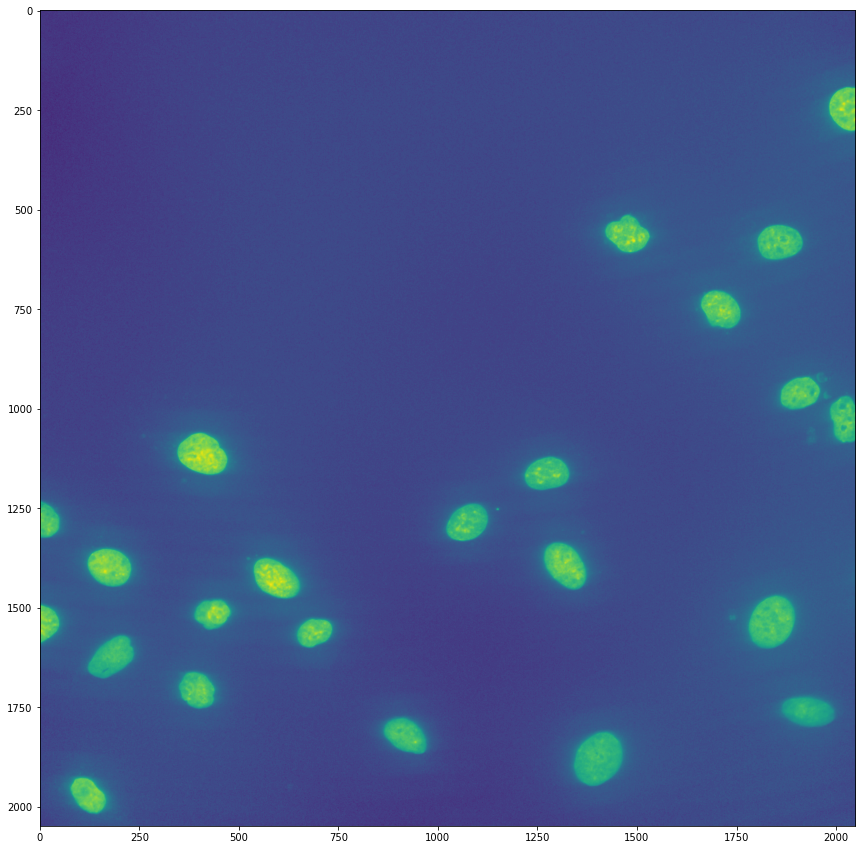
\includegraphics[width=0.3\textwidth]{wavelength_1.png}
        }
        \subfloat[Nuclei Mask]{
            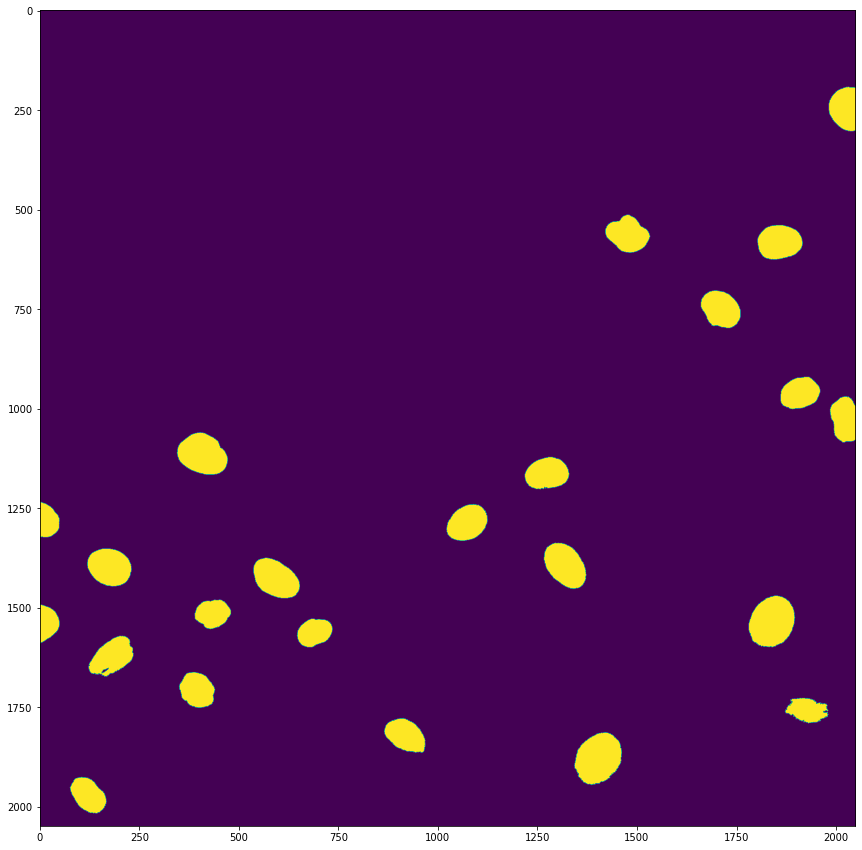
\includegraphics[width=0.3\textwidth]{nuclei_mask.png}
        }
    }\hfill{
        \subfloat[Wavelength 3]{
            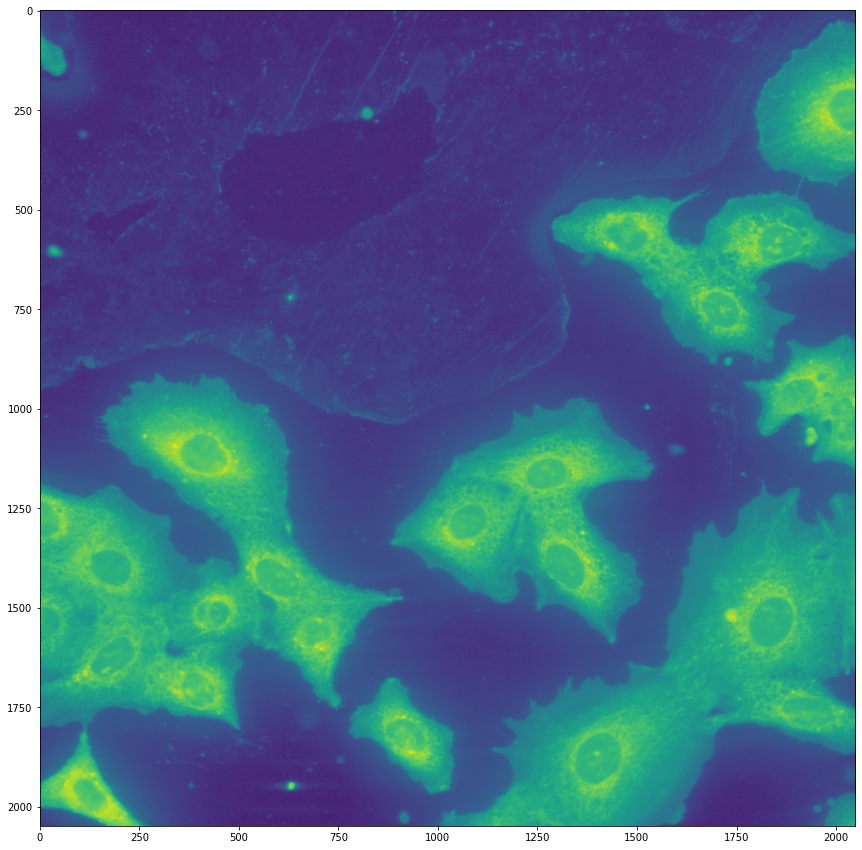
\includegraphics[width=0.3\textwidth]{wavelength_3.png}
        }
        \subfloat[Cytoplasm Mask]{
            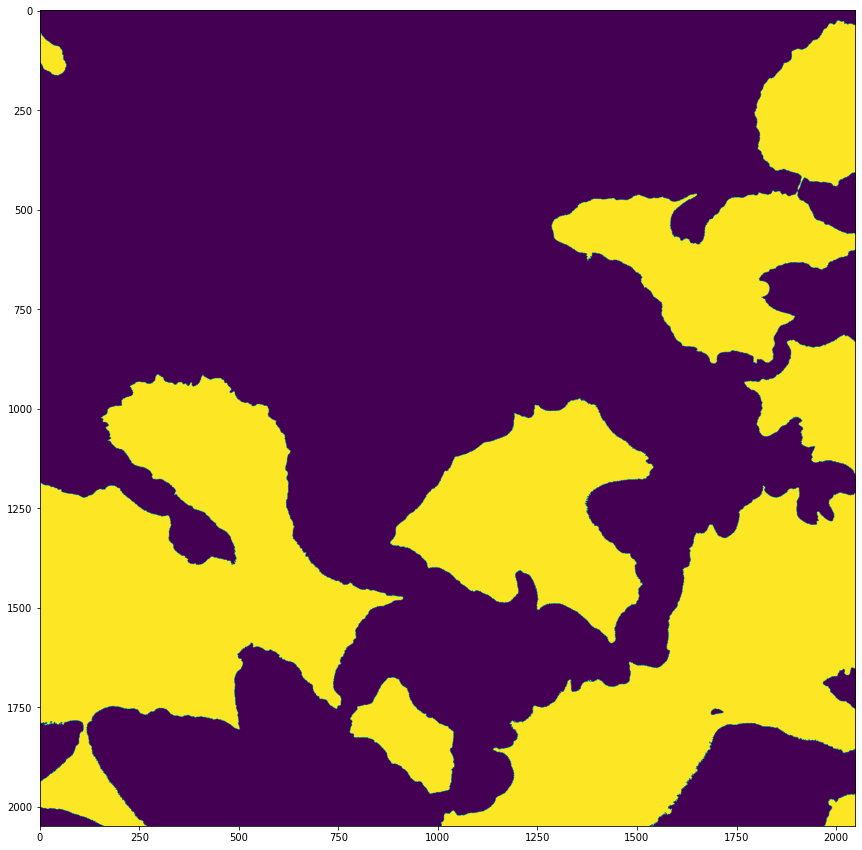
\includegraphics[width=0.3\textwidth]{cytoplasm_mask.png}
        }
    }\hfill{
        \subfloat[Segmented Cells with Nuclei]{
            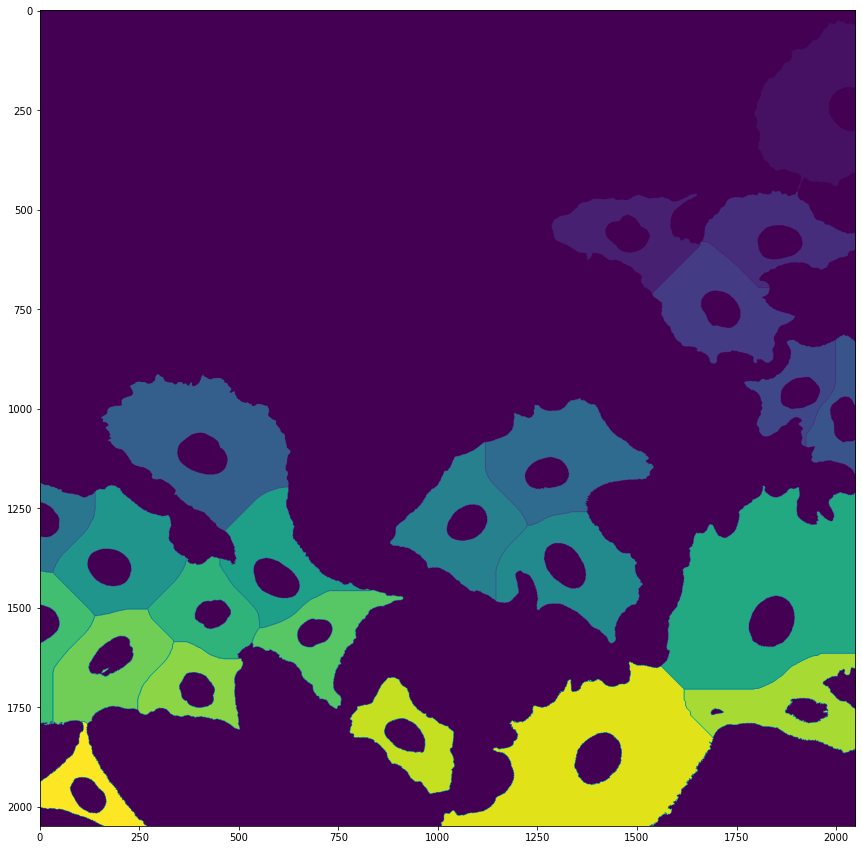
\includegraphics[width=0.3\textwidth]{combined_mask.png}
        }
        \subfloat[Mask]{
            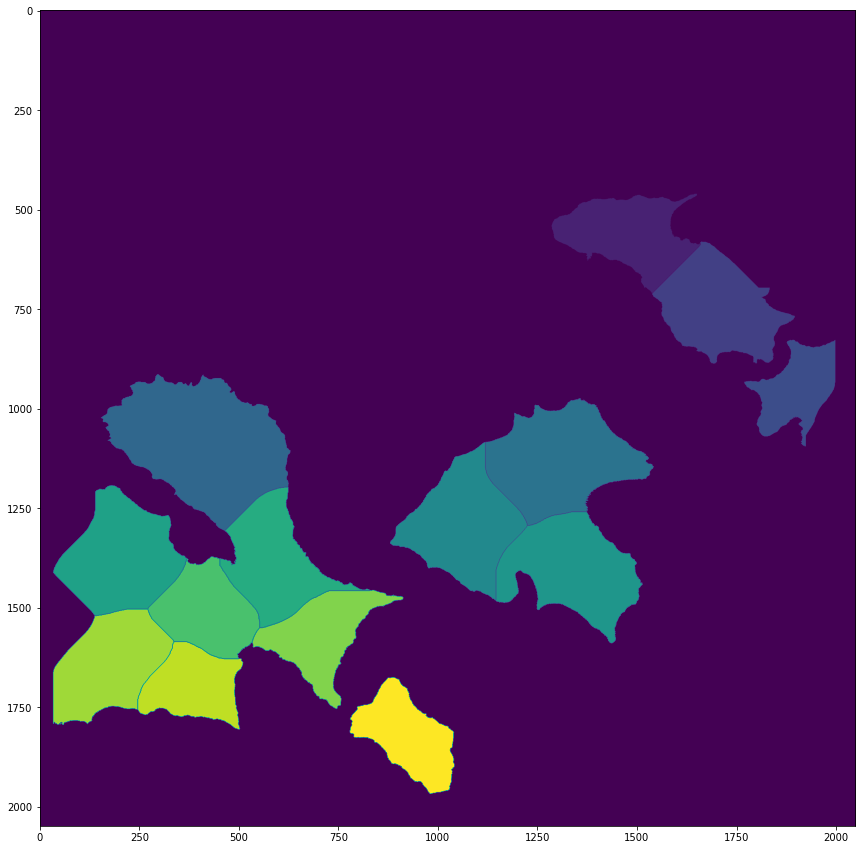
\includegraphics[width=0.3\textwidth]{final_mask.png}
        }
    }\caption{Full Masking Process}
    \label{fig:masking_process}
\end{figure}

A major impediment to accurate blob detection was the presence of overly bright cells in images that
would get recognized as containing multiple blobs due to their high pixel intensity despite not containing
blobs. An example of this is shown in Figure\ref{fig:bright_spot}. In order to prevent this from happening, pixels with intensity greater than 5 standard deviations
from the mean of the image were selected and a morphological opening was performed on the resulting 
mask. The result was a mask that contained an area indicated where pixels were abnormally bright 
but did not include condensates that were overly bright. The detection of the overly bright areas
but not overly bright condensates was accomplished using morphological opening; morphological
opening removed regions from the outlier mask that were smaller than a constant such that they would
not be identified as abnormalities. The full outlier removal process is 
shown in Figure~\ref{fig:outlier_removal}.

\begin{figure}[H]
    \centering
    {
        \subfloat[Wavelength 2 with Bright Cell]{
            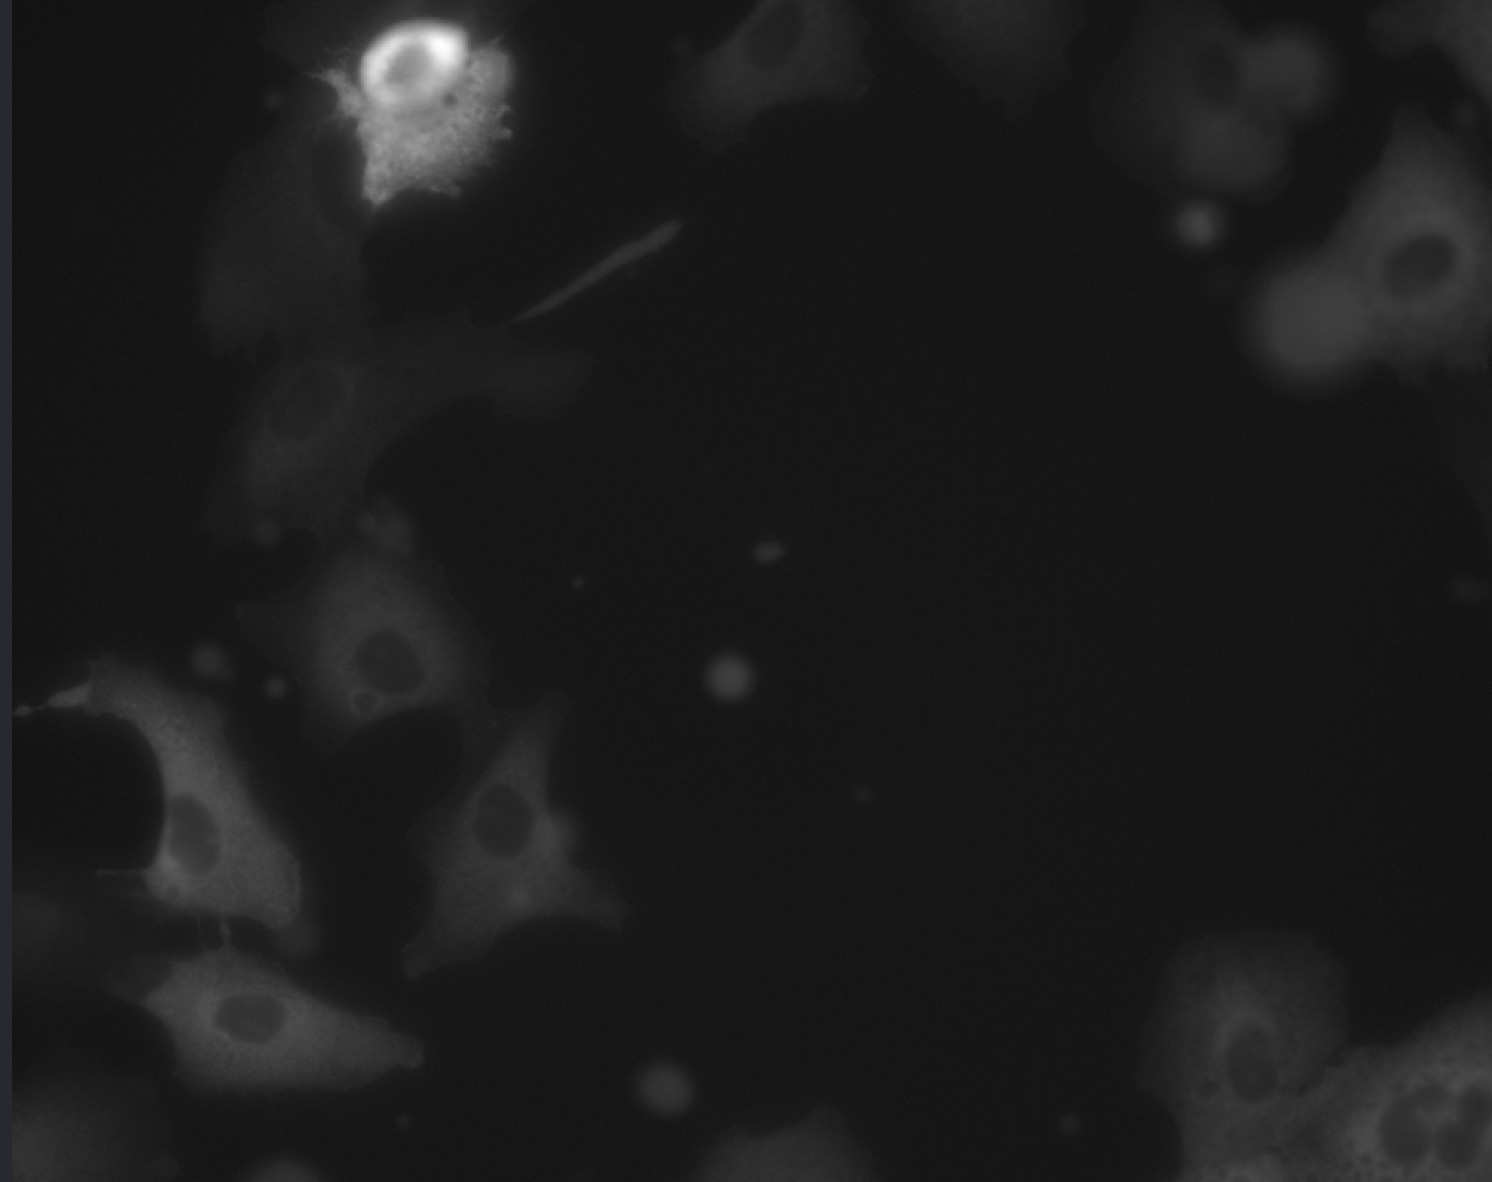
\includegraphics[width=0.5\textwidth]{bright_spot.png}
        }
    }
    {
        \subfloat[Effect on Predicted Labels]{
            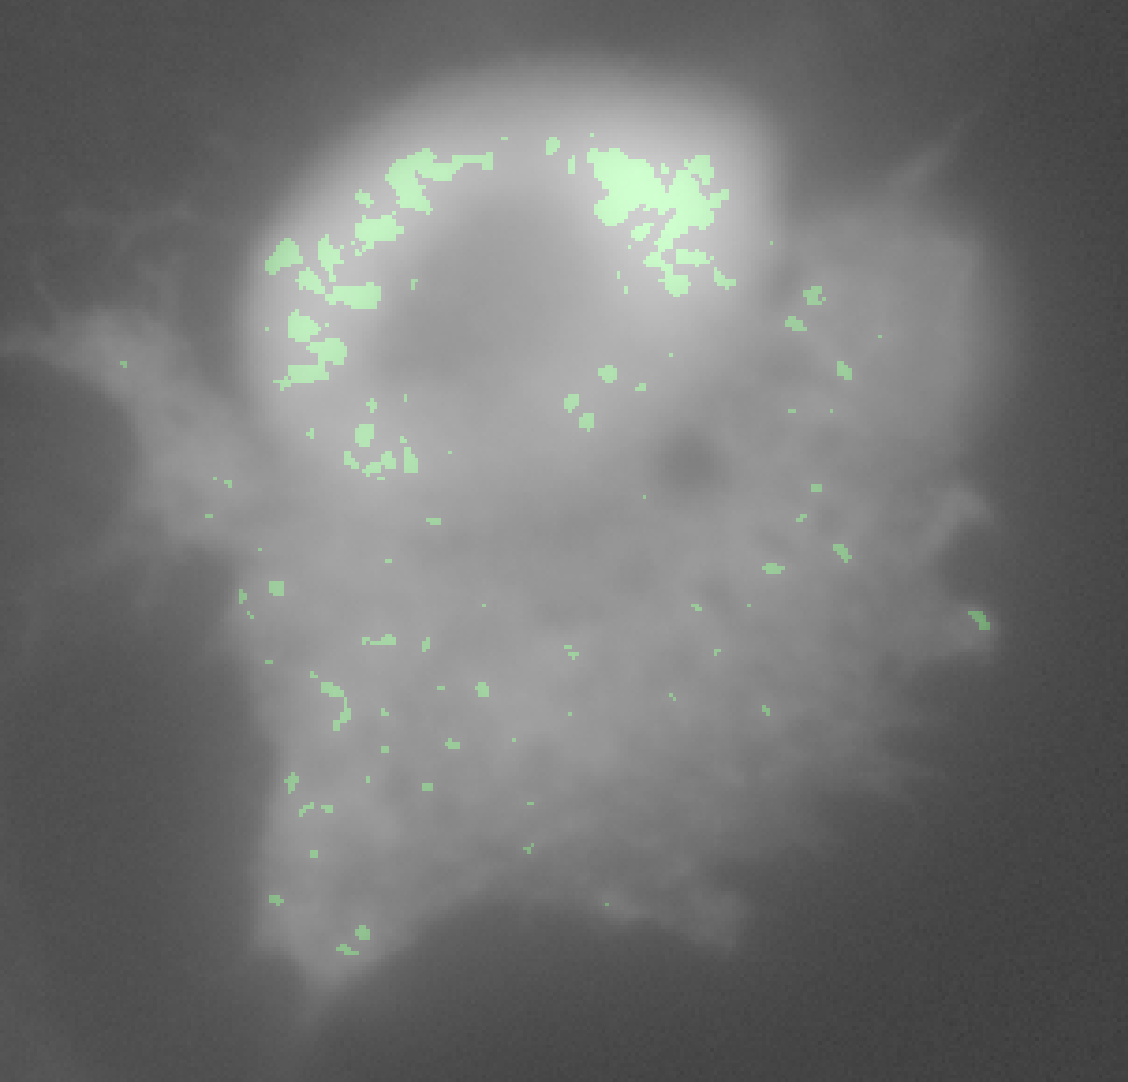
\includegraphics[width=0.5\textwidth]{bright_spot_labels.png}
        }
    }\caption{Bright Spot and Effect on Prediction}
    \label{fig:bright_spot}
\end{figure}


\begin{figure}[H]
    \centering
    {
        \subfloat[Well Site with Bright Spot]{
            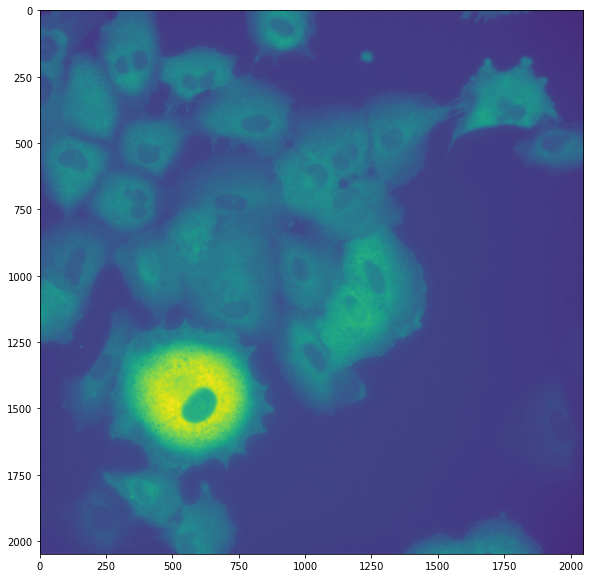
\includegraphics[width=0.3\textwidth]{bright_wellsite.png}
        }
        \subfloat[Outlier Mask]{
            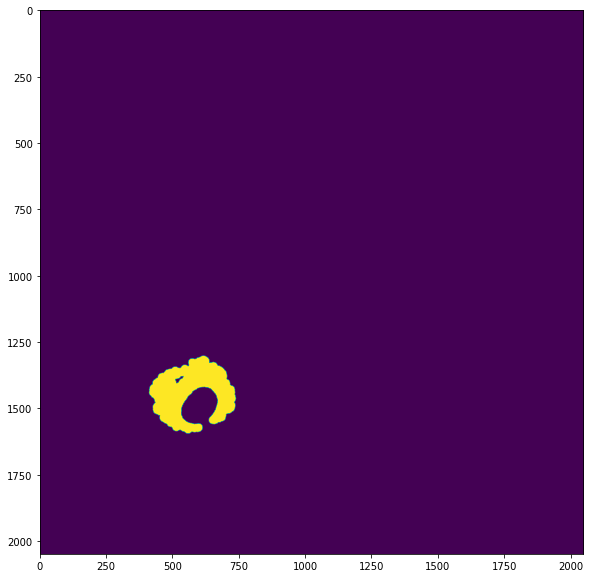
\includegraphics[width=0.3\textwidth]{bright_wellsite_outlier.png}
        }
    }\hfill{
        \subfloat[Mask Prior to Removal]{
            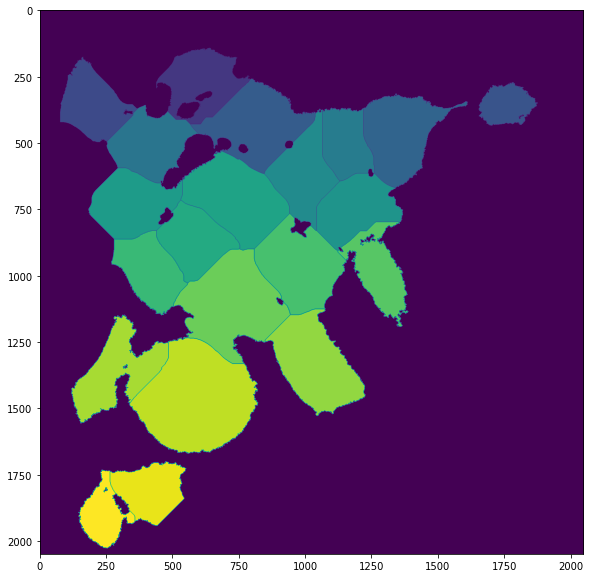
\includegraphics[width=0.3\textwidth]{bright_wellsite_premask.png}
        }
        \subfloat[Final Mask]{
            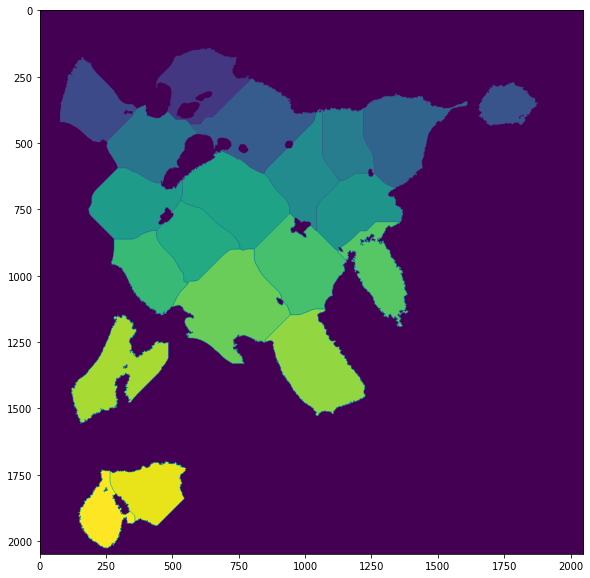
\includegraphics[width=0.3\textwidth]{bright_wellsite_mask.png}
        }
    }\caption{Outlier Removal Process}
    \label{fig:outlier_removal}
\end{figure}


\section{Feature Selection}

Labeling of images was accomplished with Napari,$^4$ a Python library for image presentation and 
labeling. An example of a labeled image portion is shown in Figure~\ref{fig:labels}. Following 
the labeling of a portion of the full data set, features were generated from the labeled pixels 
in two ways. The first way was to apply Gaussian blurring, which gave each pixel information on 
the intensities of nearby pixels in differing ranges. The second was to, in addition to Gaussian
blurring, calculate the eigenvalues of the Hessian matrix of the image and append their sum
for each set of eigenvalues calculated. This is equivalent to the calculation of the Laplacian of
the Gaussian blurred image. These two feature extraction methods were done with for varying 
variances in the Gaussian blur. Through experimentation, four values for the variance in the 
Gaussian filter were used. 

Figure~\ref{fig:gaussian_blurring} shows the application of Gaussian
blurring to a zoomed-in portion of an image. We refer to these as the intensity features of the image,
as the information they provide on the pixel is concerned mainly with intensity at the pixel and 
in pixels surrounding it.

Figure~\ref{fig:hessian} shows the component gradients of the Hessian matrix and their 
respective eigenvalues. The sum of these was calculated for each variance in the Gaussian blur
such that there were four features for each pixel. Figure~\ref{fig:texture} shows the difference
in these eigenvalues for differing values of the variance of the Gaussian blur. We refer to these
features as texture features as they are concerned with how rapidly intensity is changing at and
around a pixel, which gives insight into the relative brightness and texture of a pixel.

\begin{figure}[H]
    \centering
    {
        {
            \subfloat[Regular Image]{
                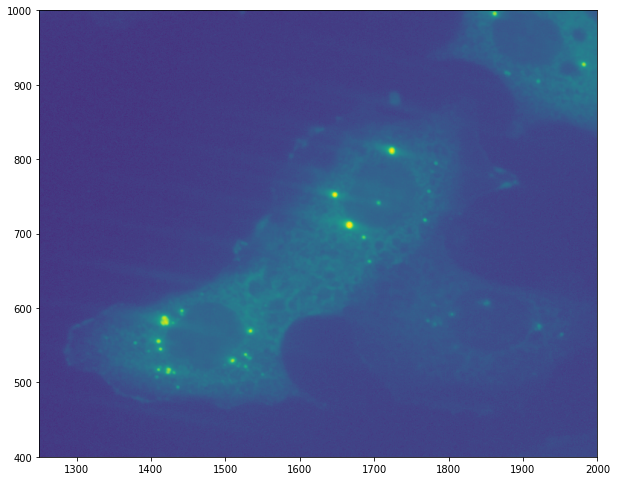
\includegraphics[width=0.3\textwidth]{zoomed.png}
            }
        }\hfill{
            \subfloat[$\sigma=1$]{
                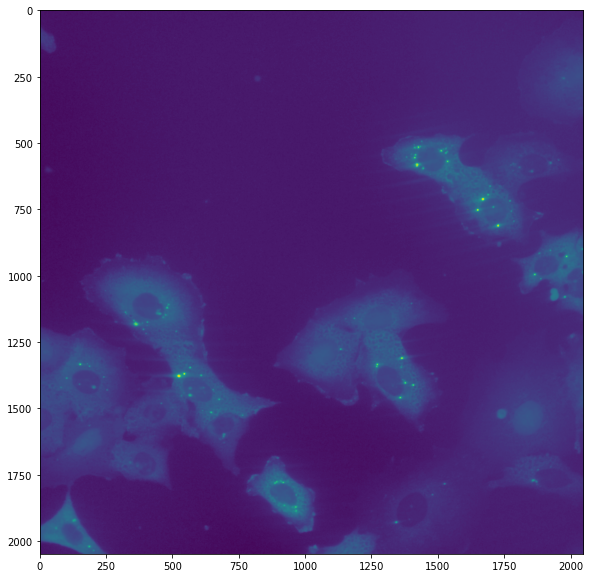
\includegraphics[width=0.3\textwidth]{gauss_blur_1.png}
            }
            \subfloat[$\sigma=2$]{
                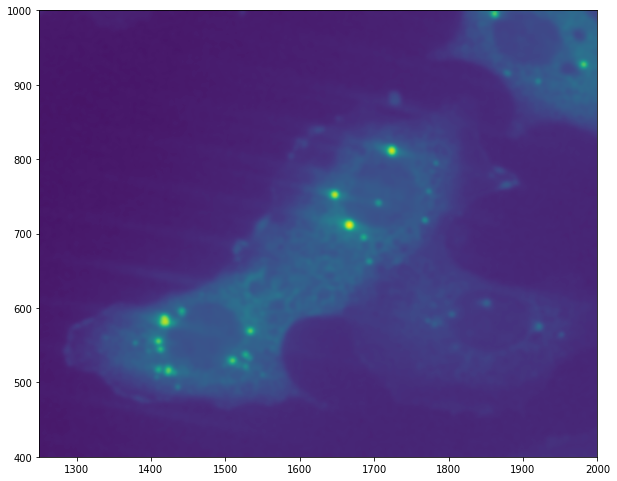
\includegraphics[width=0.3\textwidth]{gauss_blur_2.png}
            }
        }\hfill{
            \subfloat[$\sigma=4$]{
                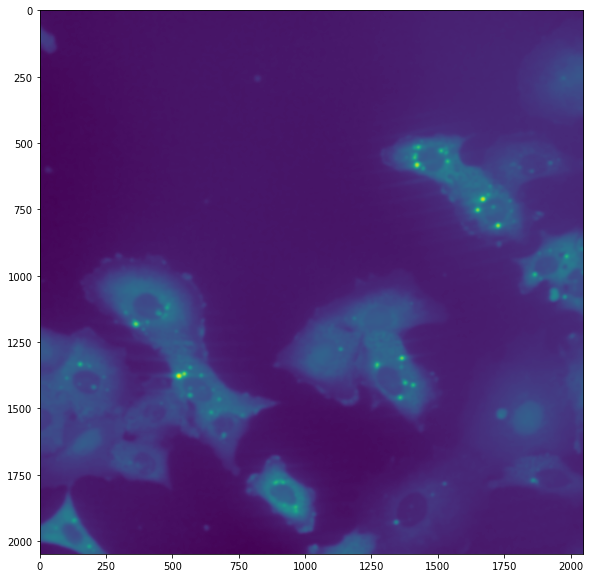
\includegraphics[width=0.3\textwidth]{gauss_blur_4.png}
            }
            \subfloat[$\sigma=8$]{
                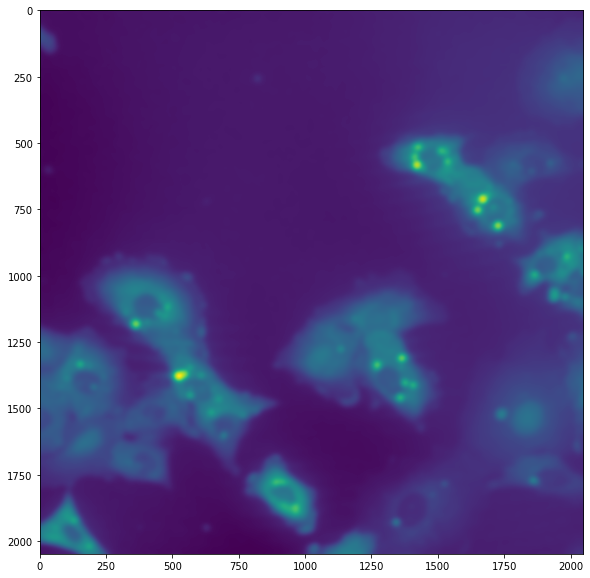
\includegraphics[width=0.3\textwidth]{gauss_blur_8.png}
            }
        }
    }\caption{Gaussian Blurring Filters}
    \label{fig:gaussian_blurring}
\end{figure}

\begin{figure}[H]
    \centering
    {
        {
            \subfloat[Regular Image]{
                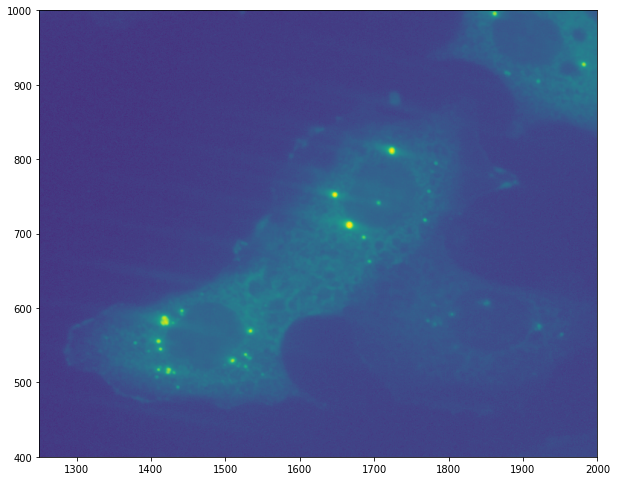
\includegraphics[width=0.3\textwidth]{zoomed.png}
            }
        }\hfill{
            \subfloat[$\sigma=4$, Hxx]{
                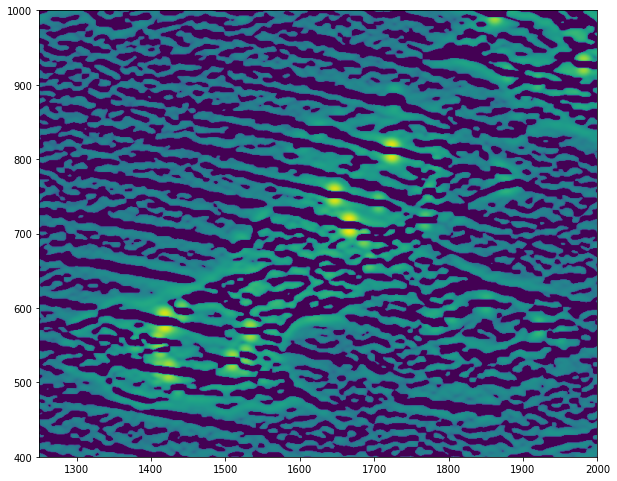
\includegraphics[width=0.3\textwidth]{zoomed_hessian_xx.png}
            }
            \subfloat[$\sigma=4$, Hxy]{
                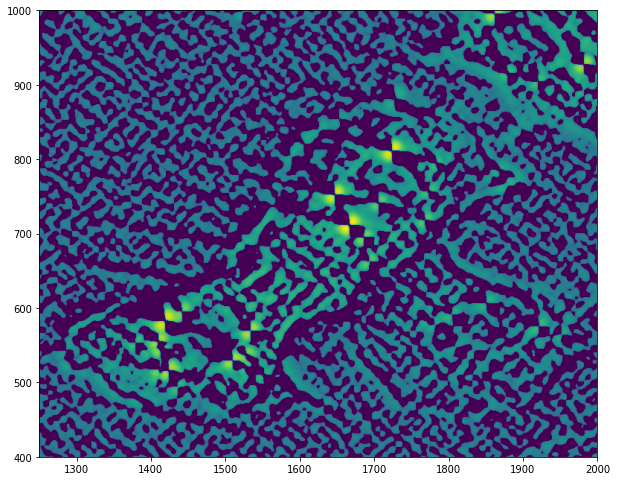
\includegraphics[width=0.3\textwidth]{zoomed_hessian_xy.png}
            }
            \subfloat[$\sigma=4$, Hyy]{
                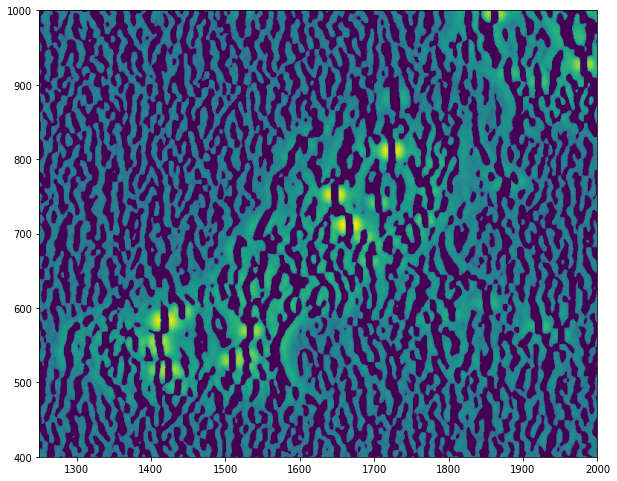
\includegraphics[width=0.3\textwidth]{zoomed_hessian_yy.png}
            }
        }\hfill{
            \subfloat[$\sigma=4$, Smaller Eigenvalues]{
                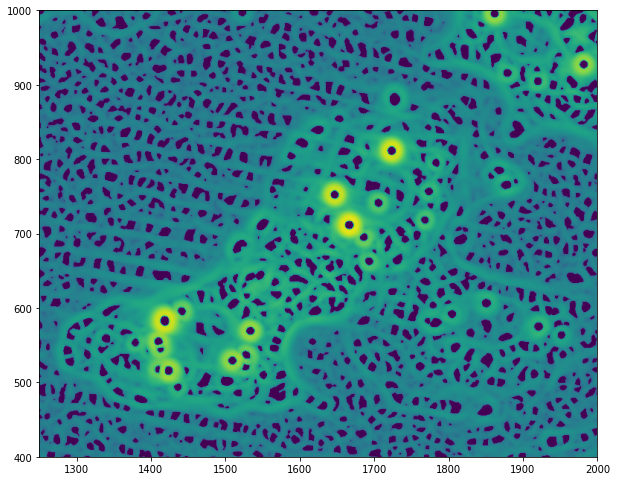
\includegraphics[width=0.3\textwidth]{zoomed_texture_4_1.png}
            }
            \subfloat[$\sigma=4$, Larger Eigenvalues]{
                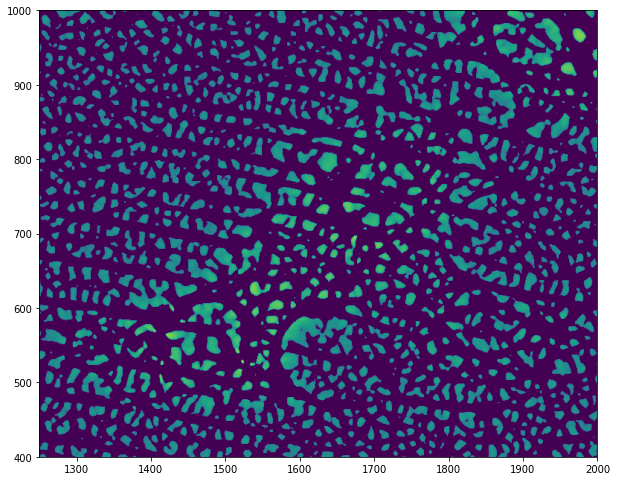
\includegraphics[width=0.3\textwidth]{zoomed_texture_4_2.png}
            }
        }
    }\caption{Gradients and Hessian Eigenvalues}
    \label{fig:hessian}
\end{figure}


\begin{figure}[H]
    \centering
    {
        {
            \subfloat[$\sigma=1$, Smaller Eigenvalues]{
                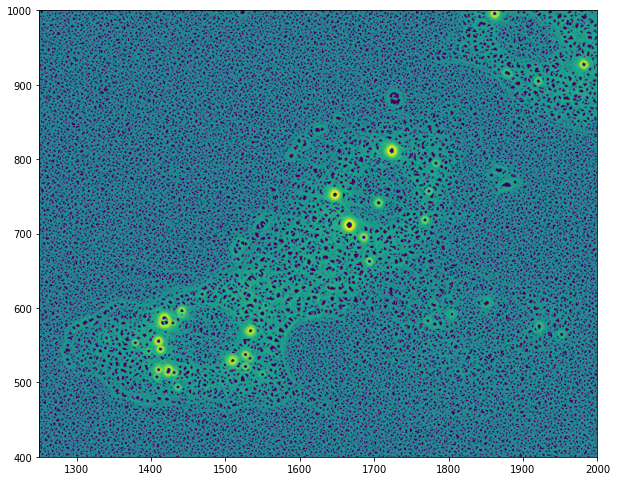
\includegraphics[width=0.3\textwidth]{zoomed_texture_1_1.png}
            }
            \subfloat[$\sigma=1$, Larger Eigenvalues]{
                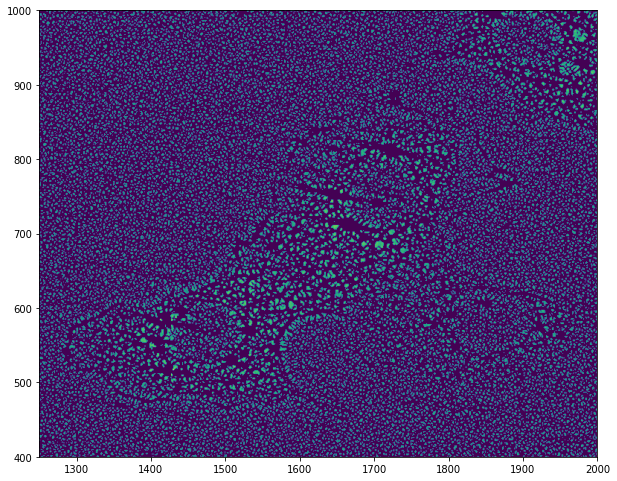
\includegraphics[width=0.3\textwidth]{zoomed_texture_1_2.png}
            }
        }\hfill{
            \subfloat[$\sigma=2$, Smaller Eigenvalues]{
                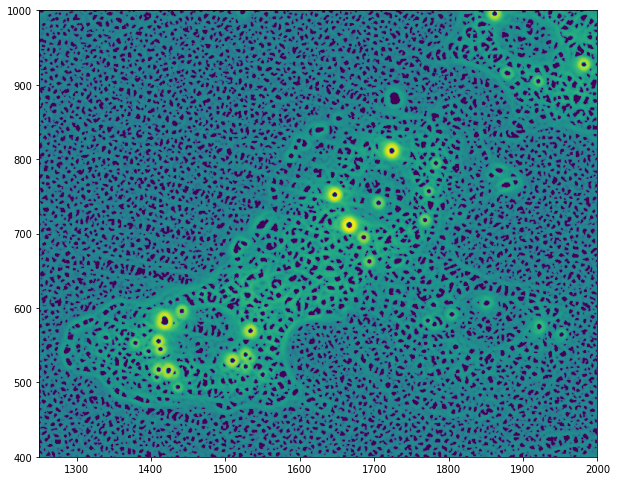
\includegraphics[width=0.3\textwidth]{zoomed_texture_2_1.png}
            }
            \subfloat[$\sigma=2$, Larger Eigenvalues]{
                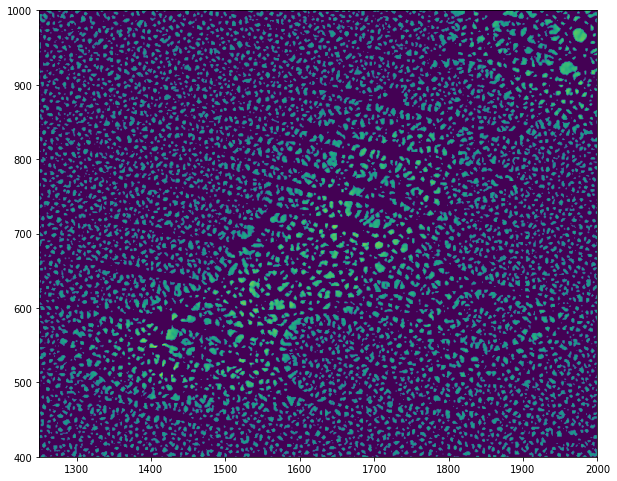
\includegraphics[width=0.3\textwidth]{zoomed_texture_2_2.png}
            }
        }\hfill{
            \subfloat[$\sigma=4$, Smaller Eigenvalues]{
                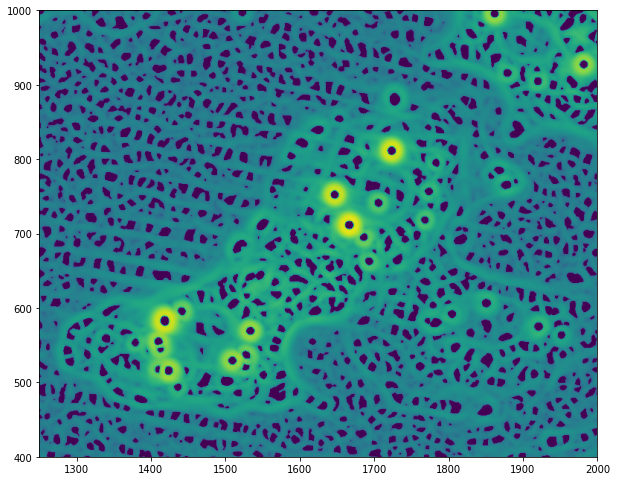
\includegraphics[width=0.3\textwidth]{zoomed_texture_4_1.png}
            }
            \subfloat[$\sigma=4$, Larger Eigenvalues]{
                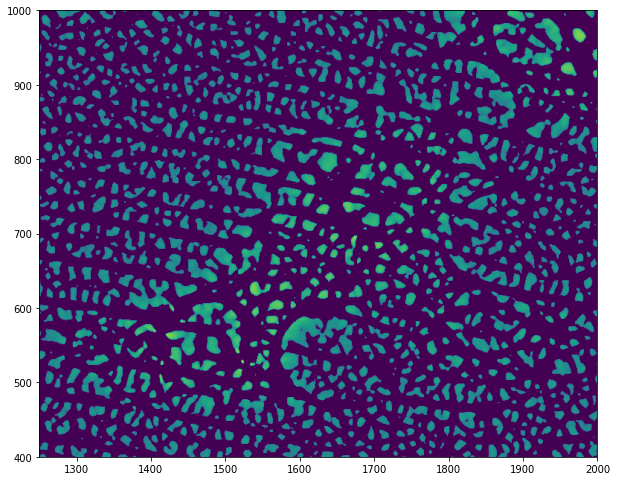
\includegraphics[width=0.3\textwidth]{zoomed_texture_4_2.png}
            }
        }\hfill{
            \subfloat[$\sigma=8$, Smaller Eigenvalues]{
                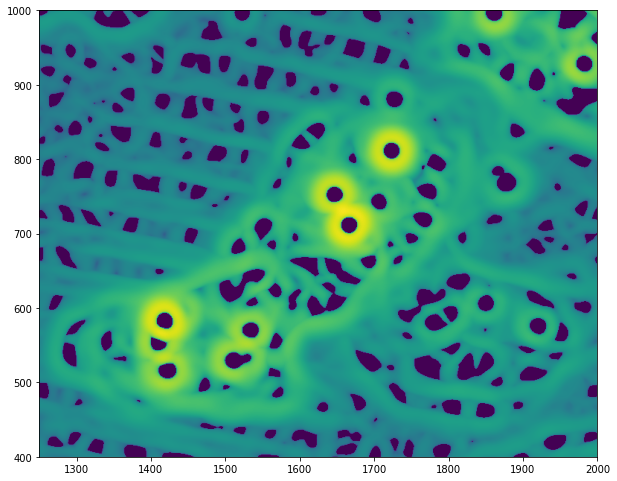
\includegraphics[width=0.3\textwidth]{zoomed_texture_8_1.png}
            }
            \subfloat[$\sigma=8$, Larger Eigenvalues]{
                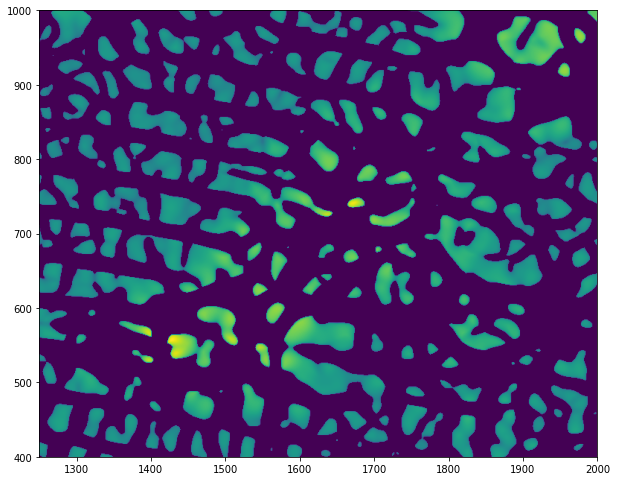
\includegraphics[width=0.3\textwidth]{zoomed_texture_8_2.png}
            }
        }
    }\caption{Full Range of Texture Filters}
    \label{fig:texture}
\end{figure}


\section{Model Selection and Results}

Two models were used for classification, Support Vector Machines and Random Forest Classifiers. 
These two were chosen for their ability to perform well given smaller training datasets. 
Differing parameters were tested for each; the parameters varied were the number of Estimators
for the random forest classifiers and the C Value for the Support Vector Machine. The resulting
balanced accuracies are displayed in Table~\ref{tab:rf_search_results} and 
Table~\ref{tab:svm_search_results}. A visualization of true vs. predicted labels is shown 
in Figure~\ref{fig:labels}.

\begin{table}[H]
    \centering
    \begin{tabular}{llrrr}
        \toprule
        \# Estimators & & Intensity Features & Texture Features \\
        \midrule
        \textsc{360} & & 0.9813 & 0.9811 \\
        \textsc{400} & & 0.9816 & 0.9813 \\
        \textsc{440} & & 0.9818 & 0.9814 \\
        \textsc{480} & & 0.9807 & 0.9816 \\
        \textsc{520} & & 0.9814 & 0.9811 \\
        \bottomrule
    \end{tabular}
    \caption{\label{tab:rf_search_results} Balanced Accuracies of Random Forest Models of Varying Estimator Counts}
\end{table}
    
\begin{table}[H]
    \centering
    \begin{tabular}{llrrr}
        \toprule
        C Value & & Intensity Features & Texture Features \\
        \midrule
        \textsc{0.001} & & 0.8388 & 0.8839 \\
        \textsc{0.01}  & & 0.8865 & 0.9330 \\
        \textsc{0.1}   & & 0.9257 & 0.9513 \\
        \textsc{1}     & & 0.9513 & 0.9611 \\
        \textsc{10}    & & 0.9701 & 0.9677 \\
        \bottomrule
    \end{tabular}
    \caption{\label{tab:svm_search_results} Balanced Accuracies of Support Vector Machine Models of Varying C Values}
\end{table}



\begin{figure}[H]
    \centering
    {
        {
            \subfloat[Drawn Labels]{
                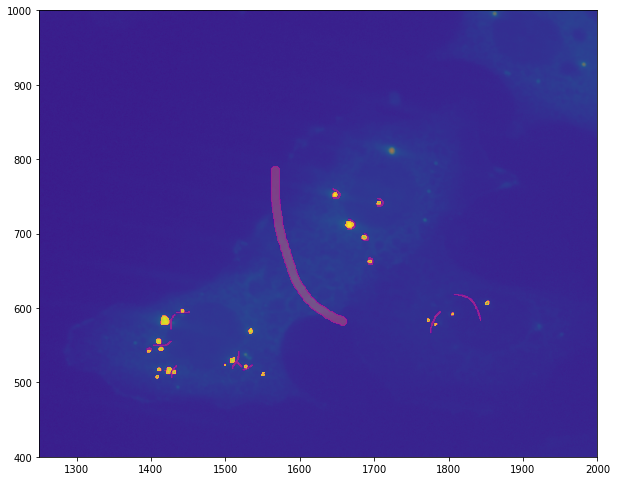
\includegraphics[width=0.5\textwidth]{y_true.png}
            }
        }
        {
            \subfloat[Prediction Result]{
                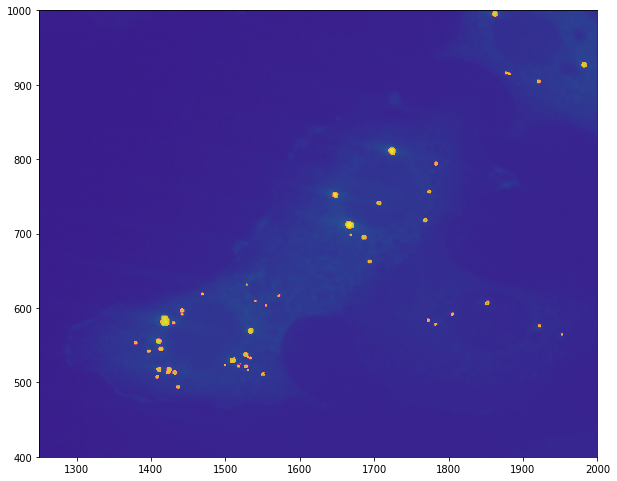
\includegraphics[width=0.5\textwidth]{y_pred.png}
            }
        }
    }\caption{True and Predicted Labels}
    \label{fig:labels}
\end{figure}

The results suggest that there is not much benefit to applying filters intended to identify edges
and texture like we did above. This is a surprising result, as virtually all traditional methods
(e.g., no machine learning) in image processing that are used to identify blobs and other features in
images rely on heavy filtering techniques. As for the accuracy of the results, the pixel
classification suggests that the methods are accurate in differentiating between pixels belonging to
and not belonging to condensates.

An important thing to note is that these accuracies represent the percentage of correctly classified
pixels weighted by each class (condensate vs. not condensate). These accuracies do not represent
the accuracy of the resulting condensate count. This is because small mis-classifications have a 
large effect on the resulting count. A single pixel misclassified as a condensate will get counted 
as a small condensate, which will heavily alter the condensate count, especially in cells 
with low/no condensates.

The full process, including pixel classification and counting using the mask calculated through
cell segmentation, is shown in Figure~\ref{fig:overlayed}. Corresponding output data, which 
includes measurements on the condensates such as intensity and area, are depicted in part in 
Figure~\ref{fig:output_data}. The resulting condensate counts of a data set of multiple wells is shown 
in Figure~\ref{fig:well_results}. These results demonstrate the difference in condensate counts in two
different types of wells, ones in which a compound was added and one in which one wasn't.

\begin{figure}[H]
    \centering
    {
        {
            {
                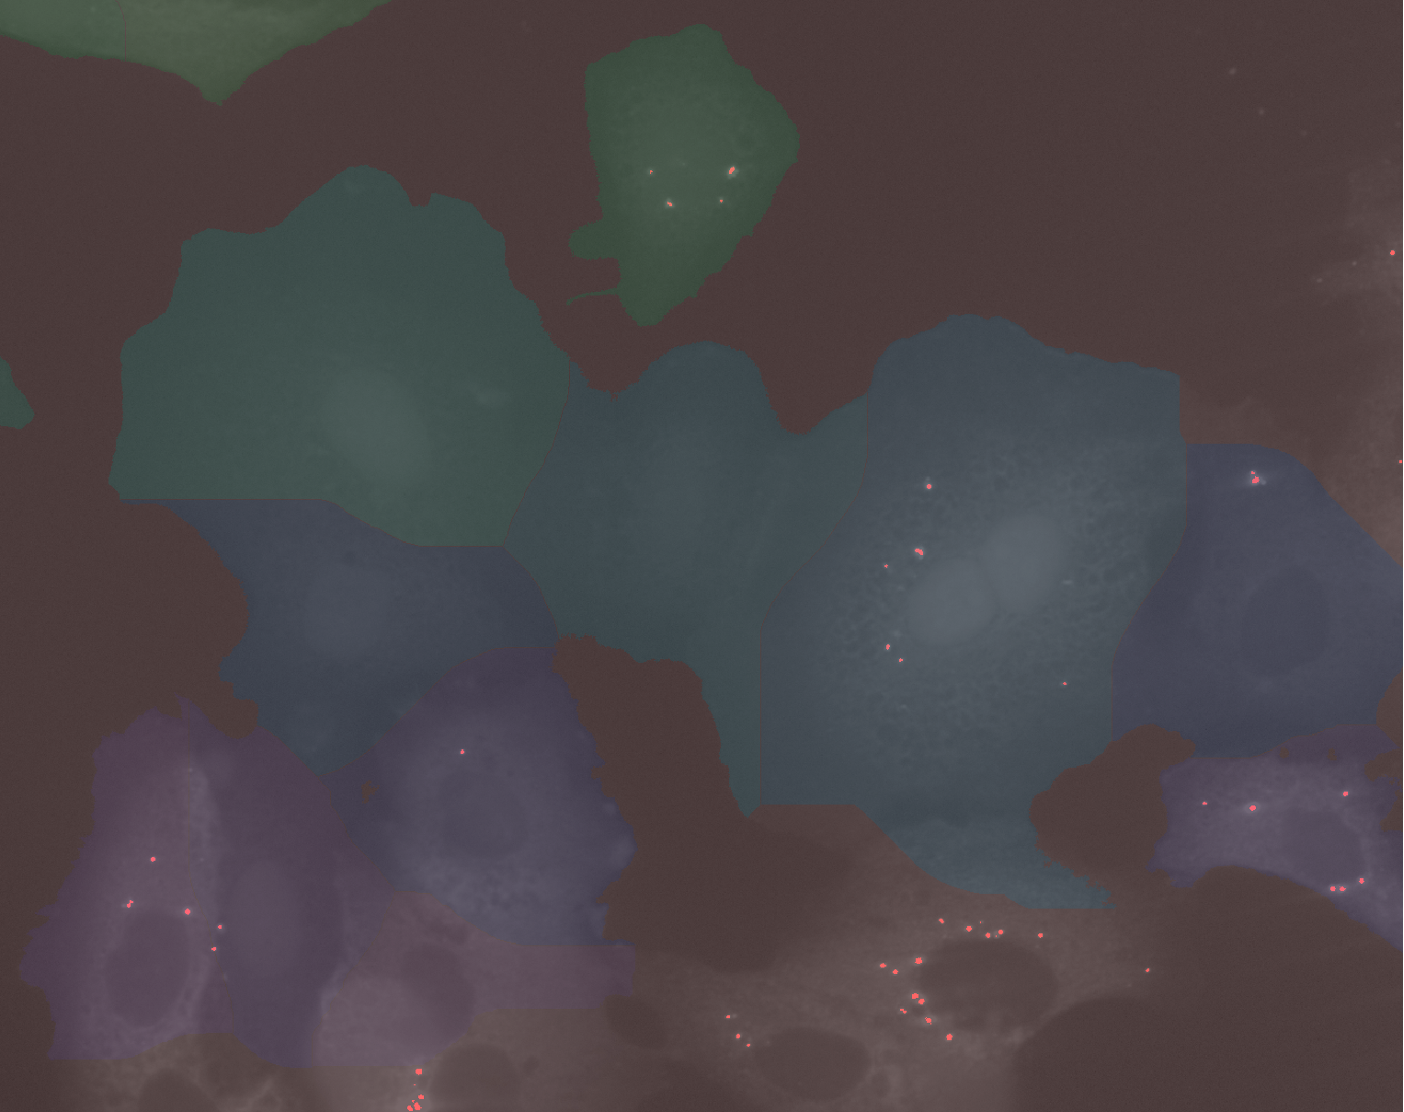
\includegraphics[width=0.9\textwidth]{overlayed.png}
            }
        }
    }\caption{Mask Overlapped with Predicted Labels}
    \label{fig:overlayed}
\end{figure}

\begin{figure}[H]
    \centering
    {
        {
            {
                \includegraphics[width=1\textwidth]{output_data.png}
            }
        }
    }\caption{Example Output Data}
    \label{fig:output_data}
\end{figure}

\begin{figure}[H]
    \centering
    {
        {
            {
                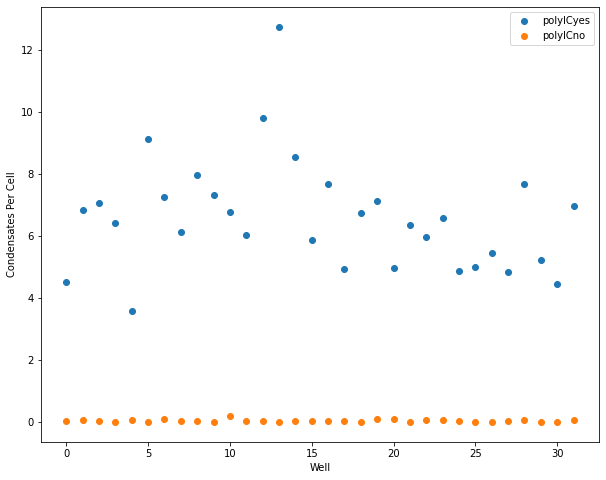
\includegraphics[width=0.7\textwidth]{well_results.png}
            }
        }
    }\caption{Counts of Wells of Different added Compounds}
    \label{fig:well_results}
\end{figure}

These results suggest that the machine learning methods were sufficient for robust qualitative assessment of 
compounds' effects on cells. 

\newpage
\section{References}

1. Berg, S., Kutra, D., Kroeger, T. et al. ilastik: interactive machine learning for (bio)image
analysis. Nat Methods 16, 1226–1232 (2019). https://doi.org/10.1038/s41592-019-0582-9 

2. Stéfan van
der Walt, Johannes L. Schönberger, Juan Nunez-Iglesias, François Boulogne, Joshua D. Warner, Neil
Yager, Emmanuelle Gouillart, Tony Yu and the scikit-image contributors. scikit-image: Image
processing in Python. PeerJ 2:e453 (2014) https://doi.org/10.7717/peerj.453 

3. Scikit-learn: Machine Learning in Python, Pedregosa et al., JMLR 12, pp. 2825-2830, 2011.

4. napari contributors (2019). napari: a multi-dimensional image viewer for python. \\
doi:10.5281/zenodo.3555620

\end{document}